\documentclass[a4paper]{article}

\usepackage[T1]{fontenc}
\usepackage[english]{babel}

\usepackage{hyperref}
\hypersetup{%
    pdfauthor = {Tobias Andersson, Victor Koronen},
    pdftitle = {ID1217: The Green Elevator},
    pdfsubject = {ID1217},
    pdfkeywords = {parallel programming},
    pdfcreator = {LaTeX with hyperref package},
    pdfproducer = {pdflatex}
}

\usepackage{graphicx}

\title{ID1217: ``The Green Elevator''}
\author{%
    Tobias Andersson <\href{mailto:tobias2@kth.se}{tobias2@kth.se}> \and
    Victor Koronen <\href{mailto:koronen@kth.se}{koronen@kth.se}>
}
\date{\today}

\begin{document}

\maketitle
\thispagestyle{empty}

\section{Introduction}

Our task was to design, implement and evaluate a controller for a simulated set
of elevators, see figure \ref{fig:hardware_control_panel}.

\begin{figure}[p]
    \centering
    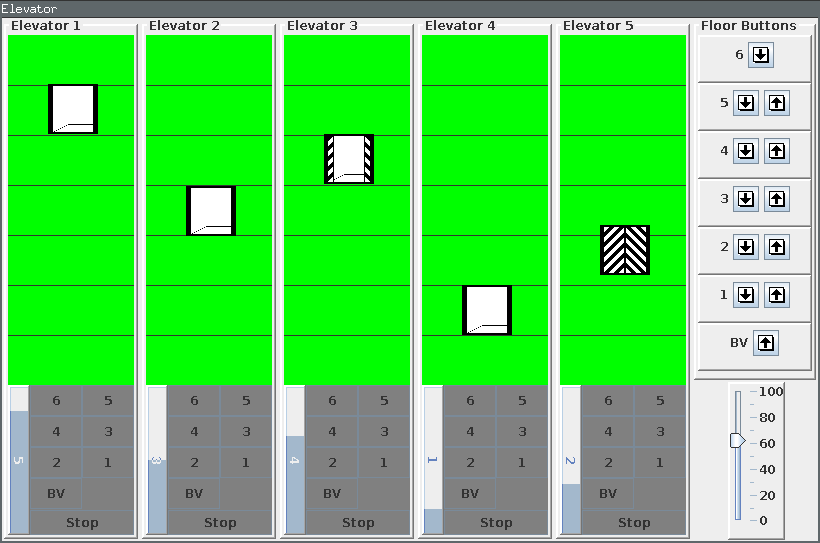
\includegraphics[width=1.0\textwidth]{images/elevators_5_6.png}
    \caption{The hardware control panel.}
    \label{fig:hardware_control_panel}
\end{figure}

\section{Implementation}

We decided to implement the controller application in Java, since it is a
language we both felt comfortable with. This also allowed us to utilize classes
from the extensive Java Standard Library and to develop the program using the
Eclipse IDE. We mainly developed the controller application in our laptops,
which both run a recent edition of the GNU/Linux Ubuntu OS.

\subsection{Structure}

The controller application consists of a set of classes with different
responsibilities.

% Describe your implementation (functions, classes, interfaces).
\begin{description}

\item[\texttt{se.kth.id1217.Main}] The main entry point to the controller
    program. Parses command line parameters, sets up the network connection and
    passes control over to \texttt{se.kth.id1217.MasterController}.

\item[\texttt{se.kth.id1217.MasterController}] Receives messages from the
    hardware. Decides which elevator should respond to floor button presses and
    passes cabin button presses onto an instance of
    \texttt{se.kth.id1217.ElevatorController}.

\item[\texttt{se.kth.id1217.ElevatorController}] The control unit for one of the
    elevators. Each elevator has a separate instance of this class. Manages the
    route for this elevator and controls the motors.

\end{description}

\subsection{Algorithms}
% Describe algorithms you have developed (chosen), synchronization or/and
% communication mechanisms you have used, and explain motivation for your design
% choices.


% the elevator controller
Each elevator controller has a queue of commands which contains tasks that has been assigned to it. This includes all button presses made inside the cabin and all floor button presses which has been assigned to it by the master controller. The elevator controller works by looking at the first item in the queue, and starts to process that task without removing it from the queue. That is done by closing the doors if needed and then starting the motors in the direction of the requested floor. Then, the controller will repeatedly sleep and poll the elevator's position and update the scale. If the elevator is at a floor, it will look if that floor is in the queue of commands. ÄR DETTA RÄTT? -> If it is, the 


% Description of an algorithm used for selection of andoing elevator to service a request (button pressing)
In order to choose which elevator to service a floor button request we developed a cost function which calculates the cost to service a request for an elevator, based on the elevator's current state and the request. When the master controller receives a floor button request, it calls the cost function of each elevator and assigns the request to the elevator with the least cost by adding it to the end of the elevator's command queue.

The cost function takes the following into account: 

whether the elevator is currently active or not, by adding a cost of COST to elevators that are currently active. This is because elevators that are not active can begin to serve the request immediately, which reduces waiting time.

if the elevator is active the task it is currently doing is taken into consideration. If the elevator is currently moving away from the floor where the request was made, a cost of COST is added, because the elevator will need to turn after it has finished its current task, which mean that waiting time will probably be long.

However, if

TODO, skriver inte om detta mer, eftersom det eventuellt kommer ändras.


 

% Explanation of synchronization mechanisms used in implementation (which mechanism, where and why).

Shared datastructures, semaphores, synchronized methods(monitors??)


\section{Evaluation}
% Present and explain your performance evaluation results, if any.

\section{Summary and conclusions}
% Give a summary of your achievements. In particular, explain briefly what you
% learned from the assignment and any problems you may have encountered. You
% are also welcome to suggest changes to the assignment in order to improve it.

\end{document}
